% The introduction of the thesis.

\chapter{Introduction}

\section{Background}

In the information enginering, XML processing as a common and popularly used
information processing technology, studies how to process XML documents and has
been intensively studied. In recent decades, the volume of information increases
dramatically, leading  an urgent demand for high-performance data processing
technologies. This change also had a greate influence to XML  processing
technology that sizes of XML documents are also increasing dramatically. For
example, Wikipedia~\cite{wiki} provides a dump service~\cite{wikipediadump} that
exports wikitext source and metadata embedded in XML documents. The sizes of the
data was less than one gigabyte before 2006. In just 10 years, it increased to
over 100 gigabytes nowadays~\cite{wikisize}. Some XML documents even reach
hundreds of gigabyte. For example, an online database of protein sequence
UniProtKB~\cite{UniProtKB} can store all the data in a single XML document sized
358 GB.

Up to the beginning of this century, studies of XML processing mainly  focused
on sequential processing~\cite{Skil97,AlJYK02,Ne02,ToGr02,HAJR03},  due to that
commonly used CPUs were mostly single-core processors. As the multiple-core CPUs
gradually became dominant gradually,  more researches shifted to parallel XML
processing  and thus more related studies were
proposed~\cite{SAFu05,PaZC08,LFLQ08,ZhPC10}.

One common topic in the field of parallel XML processing is the parallelization
of XPath~\cite{xpath} queries over XML documents. The basic idea of parallelize
is to divide an XML document into multiple parts and process queries separately
in parallel. One key problem of the parallelization is how to deal with the
hierarchical structure that is the intrinsic characteristic of each XML
document. This characteristic plays a very important role in parallel XML
document processing, forcing us to deal with the connections of the divided
parts after splitting. 

To address the above difficulty, many approaches had been proposed~\cite{JLWO03,
	SAFu05,NEMH07,BuLM08,Mats09, ZhPC10,ChLW13,HaMa16}. Most of these approaches
tend to represent XML document as trees and preserve them in memory, then
parallelizing XML processing on these trees, which usually utilize multi-thread
techniques processed in a shared memory where all the threads are able to access
the shared XML data. However, these studies discuss the parallelization of XPath
queries only on the a whole tree (or a number of whole trees) without
considering how to divide them. Thus, they are not suitable for distribued XML
document processing.

Another common approach of XML processing is to exploit database techniques. XML
processing in databases has also been widely studied~\cite{fong2001converting,
	meier2002exist, jagadish2002timber,jiang2002xparent,PCSS04}. Common database
techniques, such as indexing~\cite{kha2001xml, wang2005sequencing,
	popovici2005sirius}, join algorithms~\cite{liang2005lax,liang2006slax,
	guha2003index}, are also valid to be applied to XML processing. Although
concurrent transactions are available in modern database engines, making it
possible and available to be applied in distribued settings, there is, to the
best of our knowledge, no existing work that studies the parallelization of
XPath queries based on XML databases in a distribued-memory environment.
Therefore,  it is not clear how to utilize the power of XML databases in
evaluating of XPath queries over large XML documents in distribted-memory
environemts.

In this study, we address the following two challenges for processing large
XML documents in distributed-memory environments.

\begin{itemize} 
	\item Parallelizing Evaluation of XPath Query using XML databases.\\  
	By dividing or rewriting an XPath queries into multiple subqueries, such
	as~\cite{BoLS09,Bord10},  we can convert the evaluation of the original query to
	the evaluation of these subqueries. However, there is a technical difficulty as
	to figure out how to parallelize the evaluation of an single query by exploiting
	existing XML database engines, particularly how to distribute an XML document to 
	multiple XML databases and process them efficiently to achieve good 
	performance gain and scalability.
	
	\item General Approach to Parallelize Evaluation of XPath Queries.\\
	When processing XML documents in distributed-memory environments, it is common
	to partition an XML document into chunks and distribute the processing of chunk
	to multiple computers. However, how to represent chunks and evaluate queries on
	them for efficient evaluation, and how to handle the communication among
	computers are still challenges for efficient XML processing. \end{itemize}

This thesis addresses the above two technical differenties. There are two
corresponding approaches proposed for both shared-memory environments and
distributed-memory environments, particularly for the latter. In the following
section, we present a ``short tour'' to illustrate the contributions of this
thesis.

\section{A Short Tour}

To address the parallelization of XPath queries in XML databases, we demonstrate
our two approaches with several examples.

The first approach involves an implmentation work of~\cite{BoLS09} proposed by
Bordawekar et al., which presented approaches to easily exploit esxisting XML
processors, such as Xalan~\cite{xalan}, to parallelize XPath queires with no
need to modify  the processors. Their approach was to partition queries in an ad
hoc manner and to merge the results of partitioned queries. Specifically, they
proposed three strategies: query partitioning, data partitioning and hybrid
partitioning. Query partitioning is to split a given query into independent
queries by using predicates, e.g., from \texttt{$q_1$[$q_2$ or $q_3$]} to
\texttt{$q_1$[$q_2$]} and \texttt{$q_1$[$q_3$]}, and from \texttt{$q_1$/$q_2$}
to \texttt{$q_1$[position() <= n]/$q_2$} and \texttt{$q_1$[position() >
	n]/$q_2$}. Data partitioning is to split a given query into a prefix query and a
suffix query, e.g., from \texttt{$q_1$/$q_2$} to prefix $q_1$ and suffix $q_2$,
and to run the suffix query in parallel on each node of the result of the prefix
query. How to merge depends on the partitioning strategies.  Since hybrid
partitioning strategy is a mix of the first two partitioning strategies, we
focus on the data partitioning and query partitioning strategies in this thesis.
For query partitioning, it depends on the relationships of subqueries in the
predicate. If we split and-/or-predicates, we have to intersect/union results.
For data partitioning, if we perform position-based query partitioning and data
partitioning, we have only to concatenate results in order. In our study, we
have developed two implementations of data-partitioning parallelization and a
implementation of query-partitioning parallelization on top of
BaseX~\cite{basex864}, which is a state-of-the-art XML database engine.

The second approach is based on a novel tree structure, called partial tree. A
partital tree is a tree strcutre for representing a chunk of an XML document so
that XPath queries can be evaluated on partial trees of an XML documents in
parallel. Partial trees can be use in both shared-memory and distributed-memory
environments. To understand what a partial tree is and how it works, we use the
following XML document as an example.

\begin{quote}\small\tt
	<A><B><C>c1</C><C>c\underline{2</C><C>c3</C><A><C>c4</C><B>}\\
	</B></A></B><A><B></B></A><B></B></A> \end{quote}

We can construct a tree as shown in Figure~\ref{fig:exampletree} for
representing the given XML document. Note that each node in the tree structure
is formed by parsing a pair of tags, the start tag and the end tag. The tags in
between a pair of tags form nodes as children or descendants of the node formed
by the pair of tags. As we know, a node in the tree structure should come from a
pair of tags, but not a single tag. Thus, here comes a question: \emph{What
	structure can a single tag represent in the tree\/}?

For example, consider the underlined part of the document in
Figure~\ref{fig:exampletree}. The corresponding nodes of tags in the underlined
part are colored gray in the figure. Note that some tags, such as the first
\verb|</C>| or the last \verb|<B>| miss their matching tags. Then, how can we
represent these tags when we parse this chunk?  Besides, A$_1$ and B$_2$ are
missing in the chunk. Therefore, how can we apply  queries to the gray part in
the figure in case we do not know the path  from it to the root of the whole
tree, i.e.  A$_1$ and B$_2$?

\begin{figure}[t]
	\centering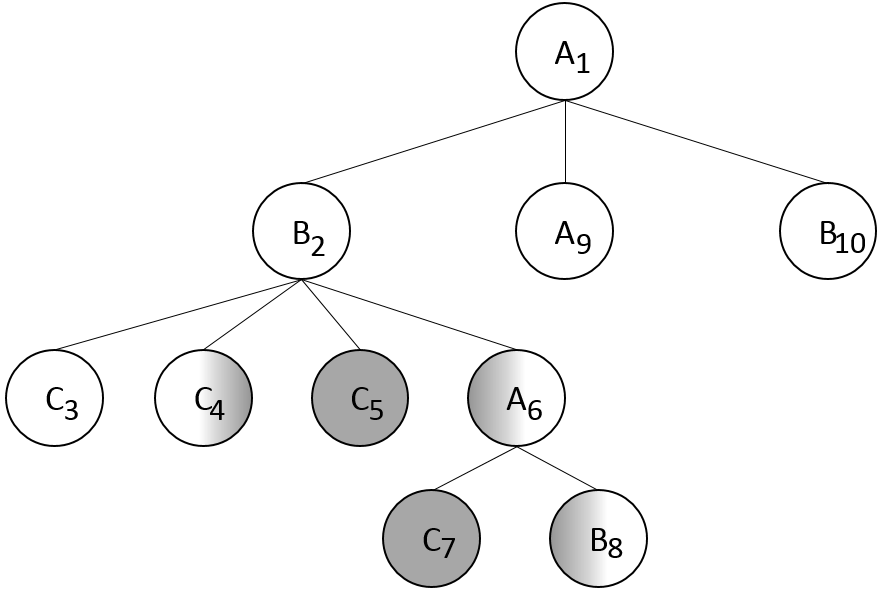
\includegraphics[scale=0.3]{figures/exampletree.png}
	\caption{An example XML tree} \label{fig:exampletree}
	\centering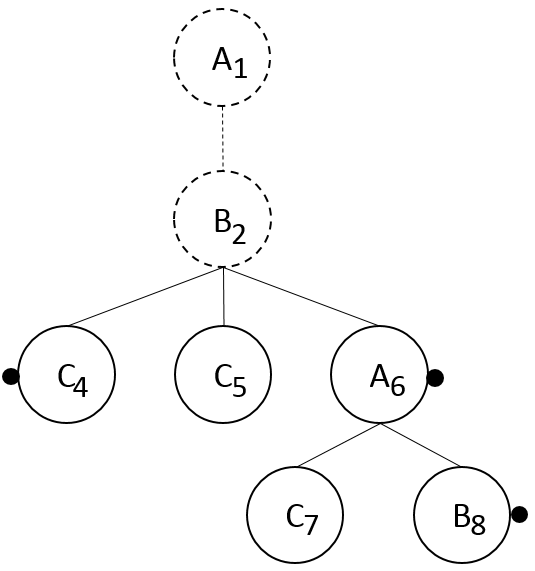
\includegraphics[scale=0.3]{figures/examplepartialtree.png}
	\caption{An example partial tree.} \label{fig:examplepartialtree}
\end{figure}

To address on the above two problems, we first proposed a novel tree structure,
called partial tree. As show in Figure 1.2.  We can create a partial tree for
the chunk. The partial tree has the information  of the missing path, i.e. A1
and B2. This tree is different from ordinary trees  because we define some
special nodes for partial tree (These special nodes with  dots in the feature
will be discussed at length in Section~\ref{sec:partialtree}).

By adding the nodes on the path from the root to the current chunk part, we are
now able to apply the queries to this partial tree based on the parent-child
relationships. We will discuss the query algorithms in
Section~\ref{sec:queryalgo}. Although partial tree is available in both
shared-/distributed- memory environments, it is more specially designed for
distributed-memory environments. This is becuase chunks of an XML documents can
distribted to multiple computers and then be parsed into partial trees for
further parallel processing.

\section{Contributions}

We consider two key contributions in the thesis.

The first contribution is the approach showing how to parallelize XPath queries
over fragmented XML documents stored in a number of XML databases, which also
involves implementations of~\cite{BoLS09}, our observations and perspectives
from the experiment results. Our implementations are designed for the
parallelization of XPath queries on top of BaseX, which is a state-of-the-art
XML database engine and XPath/XQuery 3.1 processor. With these implementations,
XPath queries can be easily parallelized by simply rewriting XPath queries with
XQuery expressions. We conduct experiments to evaluate our implementations and
the results showed that these implementations achieved significant speedups over
XML documents sized several gigabytes. Besides the experiment results, we also
present significant observations and perspectives from the experiment results.

The second contribution is the design of a novel tree structure, called partial
tree, for parallel XML processing. With this tree structure, we can split an XML
document into multiple chunks and represent each of the chunks with partial
trees. We also design a series of algorithms for evaluating queries over these
partial trees. Since the partial trees are created from separated chunks, we can
distribute these chunks to computer clusters. In this way, we can run queries on
them in distributed memory environments. We also proposed an efficient
implementation of partial tree. Based on indexing techniques, we developed a
indexing scheme, called BFS-array index along with grouped index. With this
indexing scheme, we can implement partial tree efficiently, in both memory
consumption and absolute query performance. The experiments showed that the
implementation can process 100s GB of XML documents with 32 EC2 computers. The
execution times were only seconds for most queries used in the experiments and
the throughput was approximately 1 GB/s.

\section{Outline}

The thesis is organized in six chapters. An introduction to this study is given
in Chapter 1. We  review the  related work in Chapter 2 and give definitions of
XML query languages in Chapter 3. We propose the idea of XPath queries on top of
BaseX in Chapter 4. We propose the new tree structure, partial tree in Chapter 5
and  we conclude the whole thesis in Chapter 6. Here are the detailed
introduction to the following Chapters.

Chatper 2

We dicuss related work in three aspects: 1) XML fragmentation, which studies how
to fragment an single XML document tree into multiple sub documents trees, 2)
parallel evaluation of XML queries, which is about how to evaluate query on
fragmented XML data, and  3) XML database techniques, which is database
technology that are  closely to our study.

Chapter 3

In this section, the definitions of XML and two XML query languages: XPath and
XQuery used in this these are introduced and defined. 

Chapter 4

We introduce our implementations of \cite{BoLS09}.  We introduce the XML
processing engine BaseX and we present our implementations. We evaluate our
implementations on two data sets and propose our observations and perspectives
from the experiment results.

Chapter 5

We present a noval tree structure, partial tree. We give the definitions of
partial tree, discuss the characteristics and design querying algorithms for
partial tree. We also propose an efficient BFS-index based implementation of
partial tree. We report the experiment results and analyze the results.

Chapter 6

We summarize this thesis and discuss the future work.
